
\usetikzlibrary{shapes, arrows, positioning}

\selectlanguage{english}

\tikzstyle{block} = [draw, rectangle,
    minimum height=3em, minimum width=4em, align=center, rounded corners = 3pt]
\tikzstyle{sum} = [draw, fill=blue!20, circle, node distance=1cm]
\tikzstyle{input} = [coordinate]
\tikzstyle{output} = [coordinate]
\tikzstyle{pinstyle} = [pin edge={to-,thin,black}]

% The block diagram code is probably more verbose than necessary
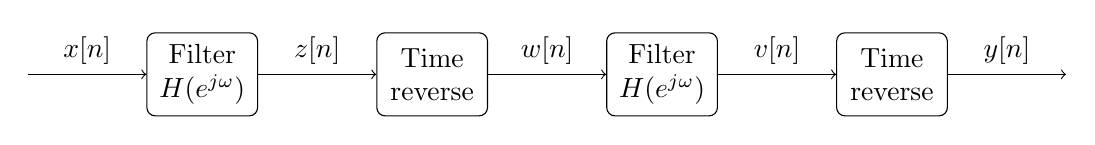
\begin{tikzpicture}[auto]
    % We start by placing the blocks
    \node [input, name=input] {};
    % \node [sum, right of=input] (sum) {};
    \node [block] (band) [right=1.5cm of input] {Filter \\ $H(e^{j\omega})$};
    \node [block] (derivative) [right=1.5 cm of band] {Time \\ reverse};
    \node [block] (squaring) [right=1.5cm of derivative] {Filter \\ $H(e^{j\omega})$};
    \node [block] (moving) [right=1.5cm of squaring] {Time \\ reverse};
    \node [output] (output) [right=1.5cm of moving] {};
    % \node [block, right=of controller, pin={[pinstyle]above:Disturbances},
    %         node distance=3cm] (system) {System of Dawn is the system};
    % We draw an edge between the controller and system block to 
    % calculate the coordinate u. We need it to place the measurement block. 
    % \draw [->] (controller) -- node[name=u] {$u$} (system);
    

    % Once the nodes are placed, connecting them is easy. 
    \draw [draw,->] (input) -- node {$x[n]$} (band);
    \draw [->] (band) -- node {$z[n]$} (derivative);
    \draw [->] (derivative) -- node {$w[n]$} (squaring);
    \draw [->] (squaring) -- node {$v[n]$} (moving);
    \draw [->] (moving) -- node [name=y] {$y[n]$}(output);
    % \draw [->] (moving) |- node {} (derivative);
    % \draw [->] (sum) -- node {$e$} (controller);
    % \draw [->] (moving) -- node [name=y]; {$y$}(output);
    % \draw [->] (y) |- (measurements);
    % \draw [->] (measurements) -| node[pos=0.99] {$-$} 
    %     node [near end] {$y_m$} (sum);
\end{tikzpicture}

\selectlanguage{greek}